\documentclass[aspectratio=43]{beamer}

\usetheme{simple}

\usepackage{lmodern}
\usepackage[scale=2]{ccicons}
\usepackage{multicol}

\usepackage[utf8]{inputenc}



% Info de la presentación
\def\edicion{XXXV}
\def\fecha{Abril 2023}

\title{Te has instalado Linux... ahora, ¿qué?} % título de la presentación
\author{Luis Daniel Casais} % autor de la presentación
\github{rajayonin} % GitHub

\institute{\edicion \ Jornadas Técnicas del GUL}
\date{\fecha}



% Cover
\titlegraphic{img/logo1.png}
\begin{document}

{
    \setbeamertemplate{footline}{}
    \begin{frame}
        \titlepage
    \end{frame}
}
\addtocounter{framenumber}{-1}


% Table of contents
\begin{frame}
    \frametitle{Tabla de contenidos}
    \begin{multicols}{2}
        \tableofcontents
    \end{multicols}
\end{frame}



% -----------------------------
% La presentación empieza aquí.
% -----------------------------


\begin{frame}
    \frametitle{Transparencias}
    \centering
    
    \begin{figure}
        
\includegraphics[width=0.5\textwidth]{img/qr-code.png}
    \end{figure}

    \href{https://github.com/rajayonin/linux-now-what}{github.com/rajayonin/linux-now-what}

\end{frame}


\section{Personalización}
% Desktop Enviroments / tiling window managers (i3) / tty
% Emuladores de terminal: kitty (bonito y simple, usa GPU), terminator (GUI friendly), alarcritty (moderno, usa GPU), iterm2 // tmux
% Shells: bash, zsh, fish
% Dotfiles: .bashrc, etc


\begin{frame}
    \frametitle{GUI (Graphical User Interface)}
    Por defecto, Linux cuenta con tres tipos principales de interfaces: dos gráficas, \textbf{Lockscreen} (pantalla de bloqueo) y \textbf{Desktop Enviroment}; y una de texto, la \textbf{TTY/shell}.\newline

    Se puede acceder a cualquiera de ellos con las siguientes combinaciones de teclas:
    \begin{itemize}
        \item \texttt{CTRL + ALT + F1}: Lockscreen
        \item \texttt{CTRL + ALT + F2}: Desktop Environment
        \item \texttt{CTRL + ALT + F3}: TTY3
        \item \texttt{CTRL + ALT + F4}: TTY4\\
        ...\newline
    \end{itemize}
    
    Cualquiera de los tres tipos son personalizables e intercambiables, ya que \textbf{LINUX ES EL AMO Y SEÑOR DE LA PERSONALIZACIÓN}.
\end{frame}

\subsection{Desktop Enviroments}

\begin{frame}
    \frametitle{Desktop Enviroments}
    Es la principal forma (moderna) de interacción con el ordenador.\\
    Todo lo que puedes ver y tocar (iconos, ventanas, \textit{toolbars}, \textit{wallpapers}, etc.) es parte del Desktop Enviroment.\newline

    Son todos intercambiables y, aunque la forma de hacerlo depende de la \textit{distro} específica, normalmente se pueden cambiar en la \textit{lockscreen}.\\
    Algunas \textit{distros} incluso te permiten elegir cual usar al instalar el SO.\newline

    Hay dos tipos principales, dependiendo de cómo manejan el uso de las ventanas: \textbf{Floating Window Managers} y \textbf{Tiling Window Managers}.
\end{frame}

\begin{frame}
    \frametitle{Floating Window Managers}
    La típica interfaz de un Sistema Operativo moderno, con ventanas "flotantes". Intuitivo y fácil de usar.\newline

    % images
    \begin{columns}[c]
        \begin{column}{0.5\textwidth}
            \begin{figure}
                \centering
                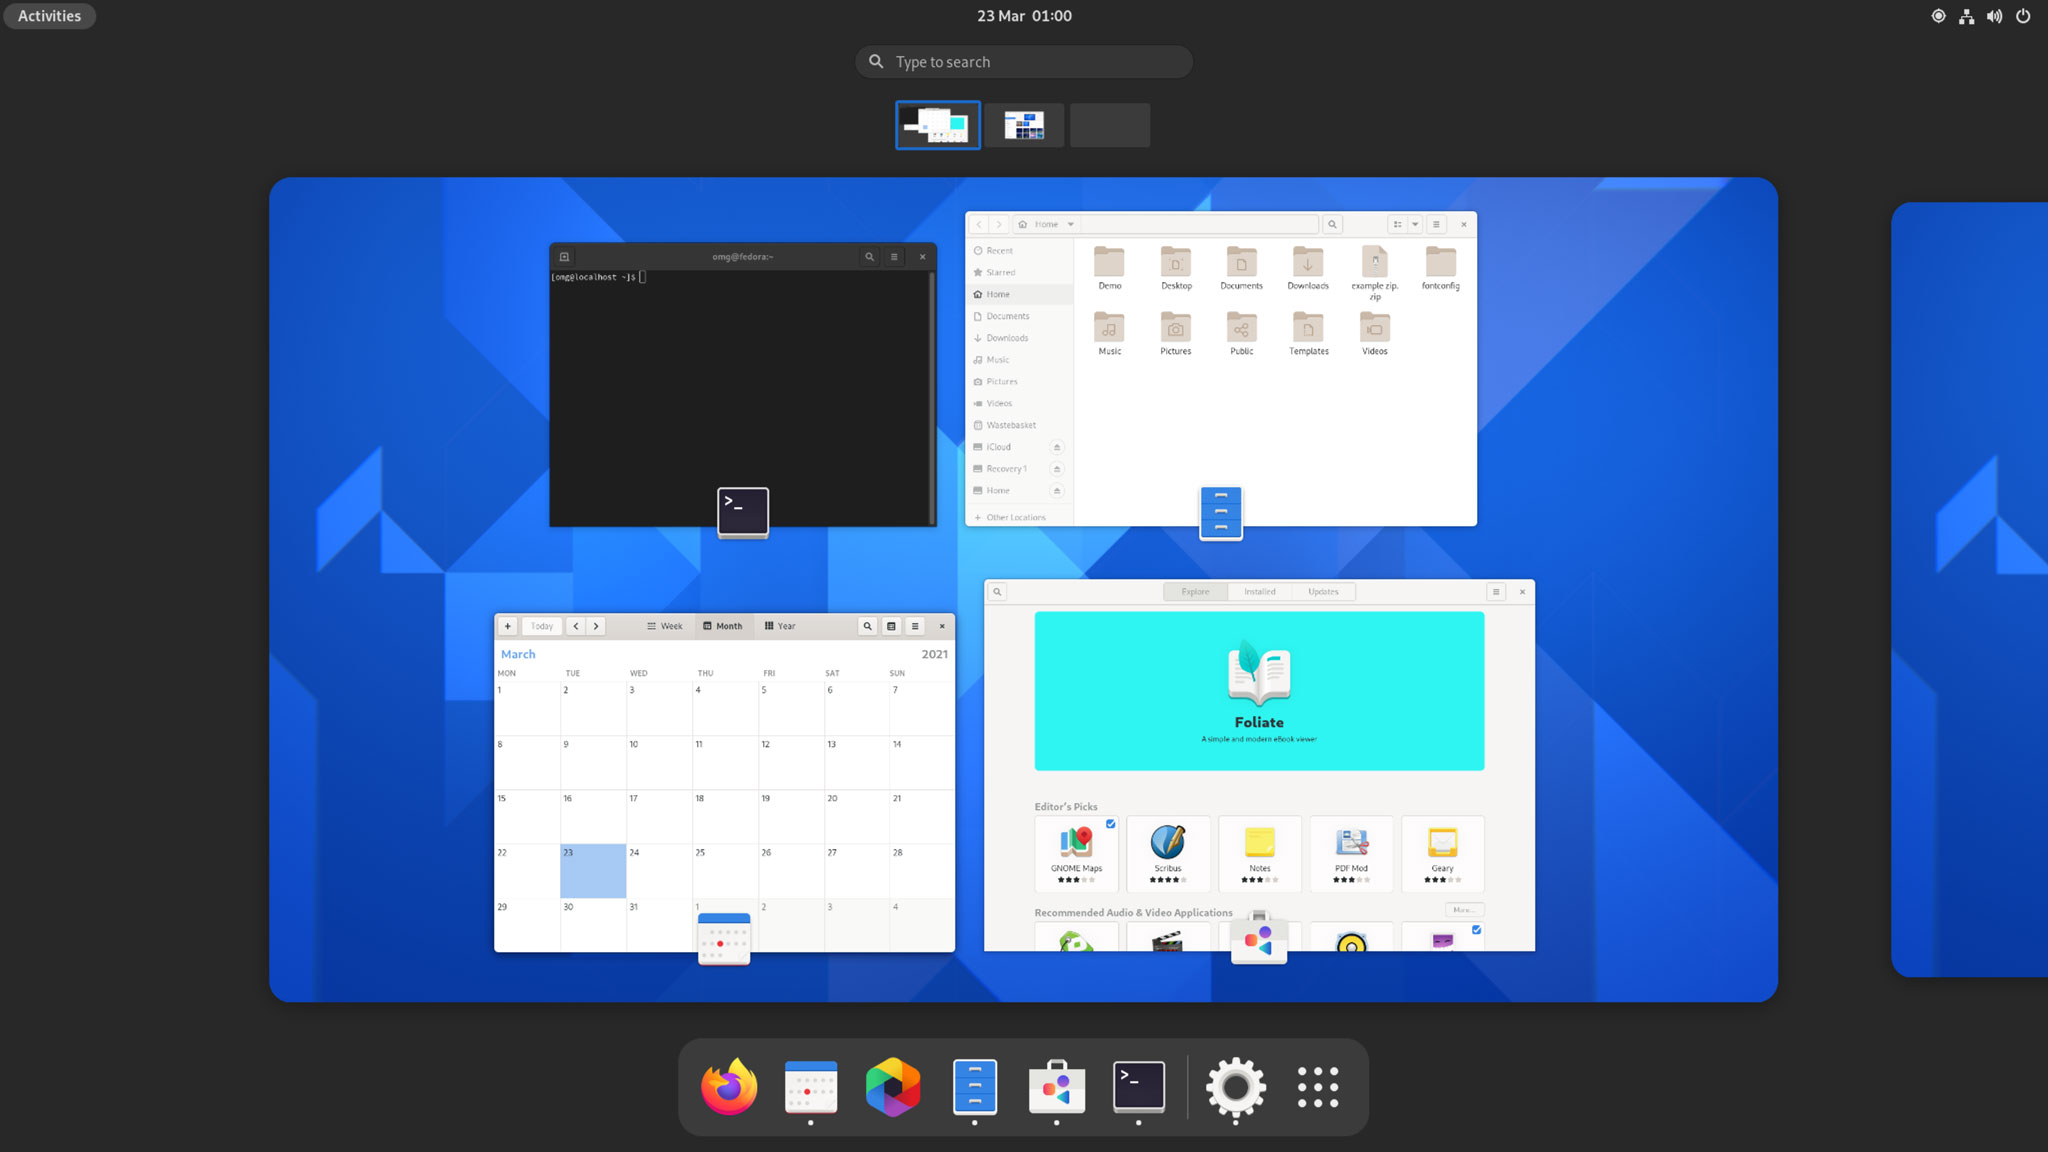
\includegraphics[width=0.9\textwidth]{img/gnome-desktop.jpg}
                \caption{\href{https://forty.gnome.org/}{Gnome 40 Desktop}}
            \end{figure}
        \end{column}
        \begin{column}{0.5\textwidth}
            \begin{figure}
                \centering
                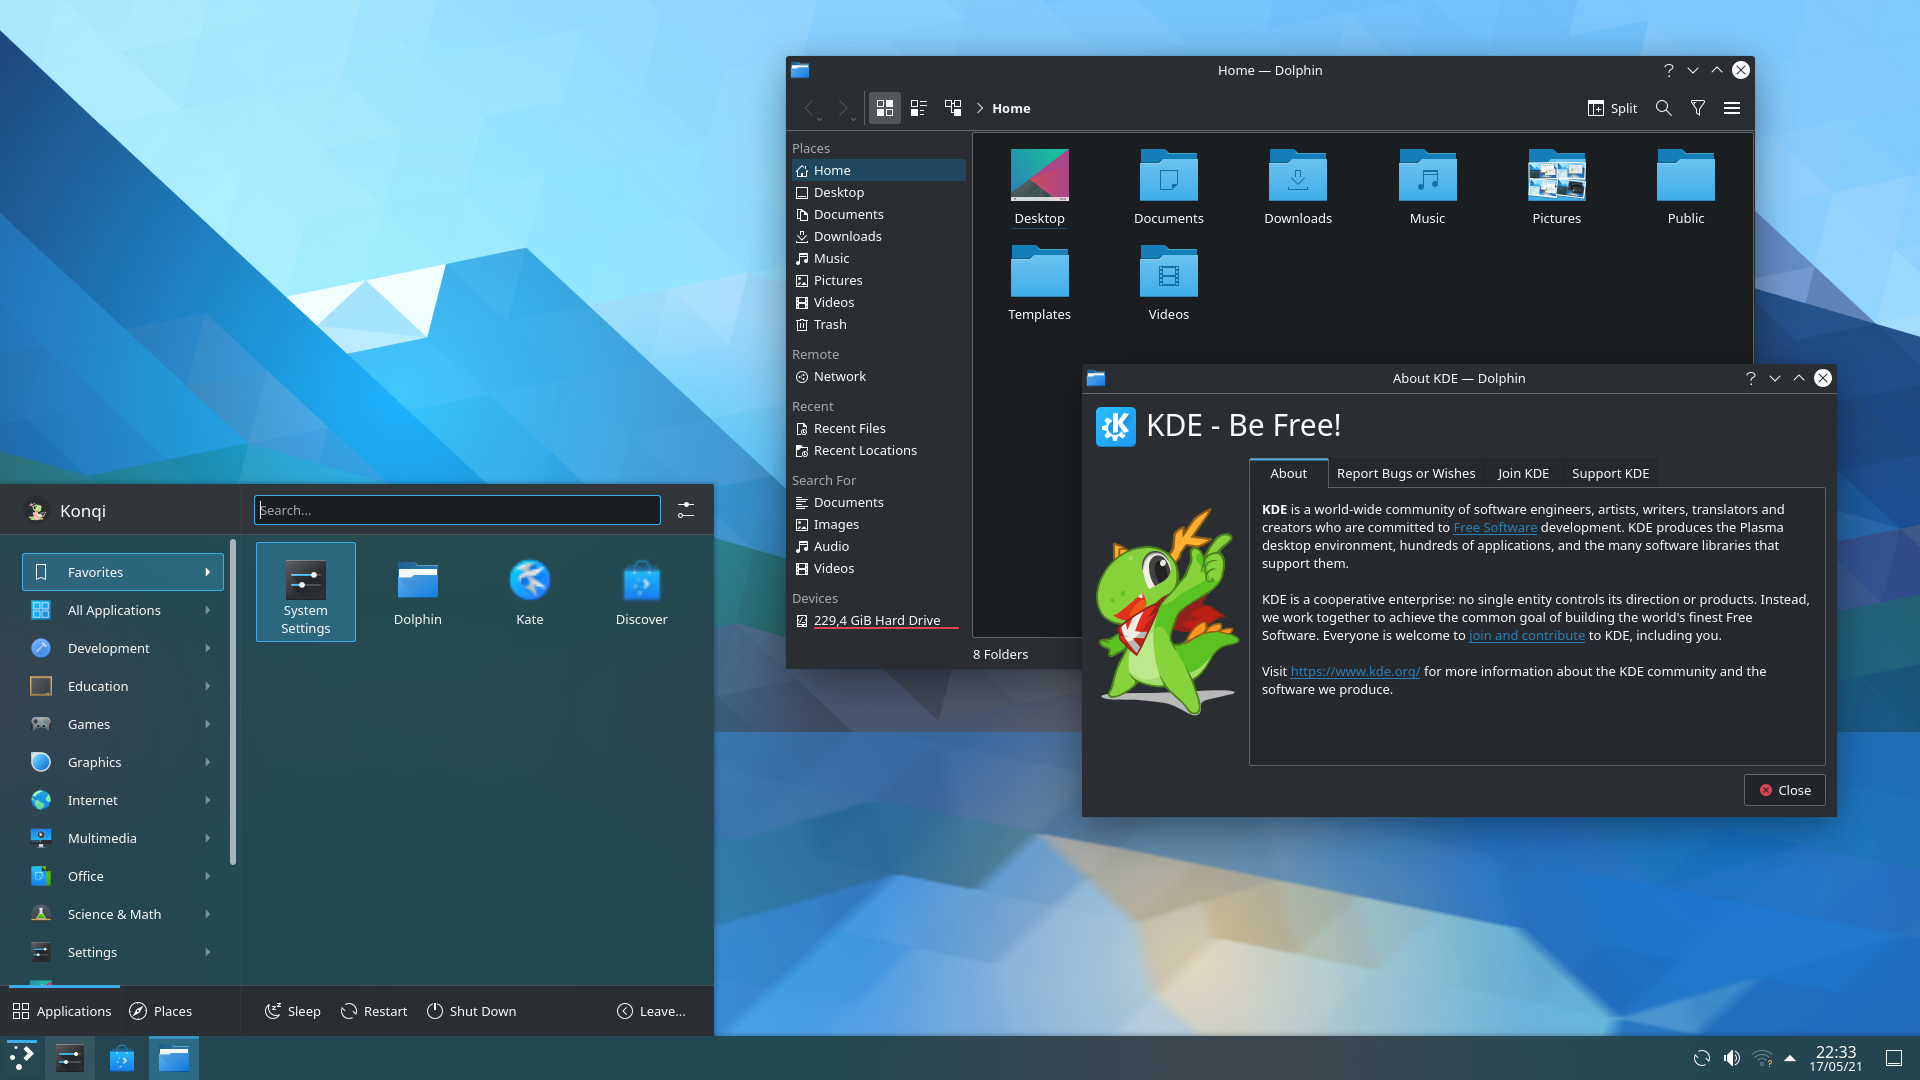
\includegraphics[width=0.9\textwidth]{img/kde_plasma.png}
                \caption{\href{https://kde.org/es/plasma-desktop/}{KDE Plasma Desktop}}
            \end{figure}
        \end{column}
    \end{columns}

\end{frame}

\begin{frame}
    \frametitle{Tiling Window Managers}
    Máximo uso del espacio de la pantalla, 100\% del tiempo (automático). Infinito control y personalización del escritorio.\\
    Todo con \textit{hotkeys} (ratón pa' qué?), pero más difícil de aprender.

    \begin{figure}
        \centering
        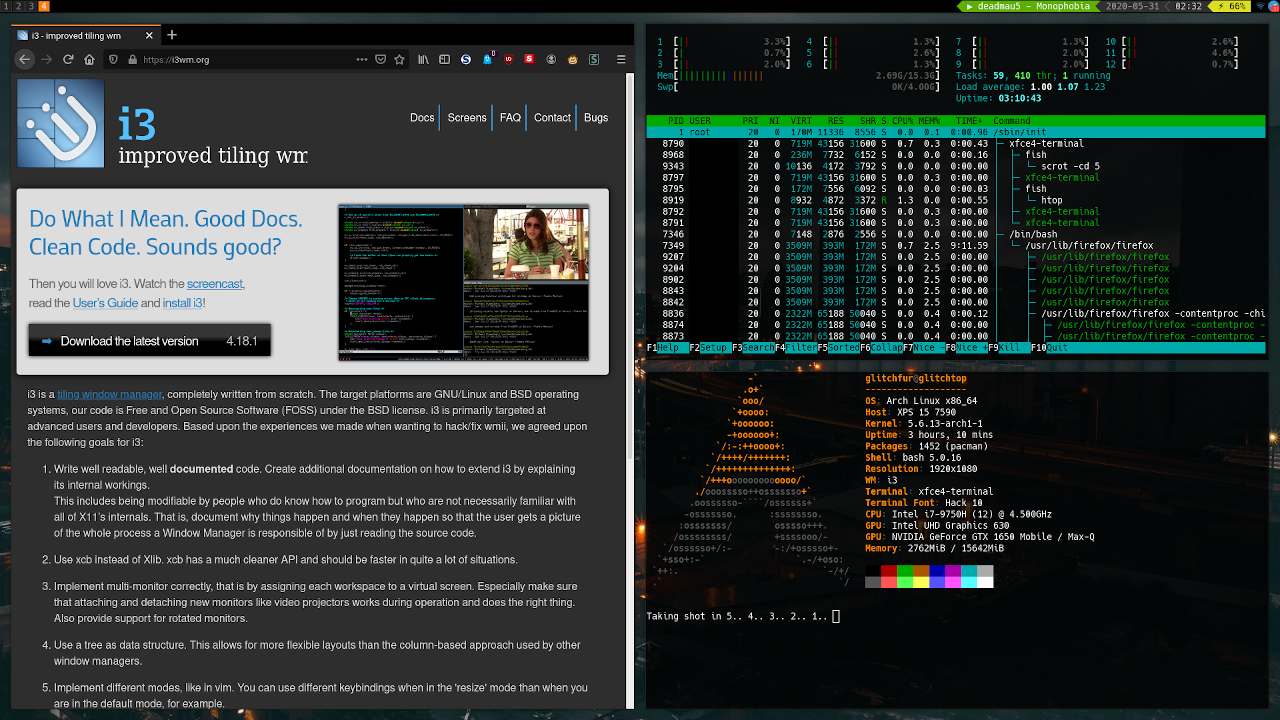
\includegraphics[width=0.6\textwidth]{img/i3_window_manager.png}
        \caption{\href{https://i3wm.org/}{i3 Window Manager}}
    \end{figure}
\end{frame}


\subsection{Emuladores de terminal}
\begin{frame}
    \frametitle{Emuladores de terminal}
    Permiten interactuar con la terminal real, y añaden muchas funcionalidades (copiar y pegar, múltiples terminales...), aparte de personalizar cosas como colores, fuentes...\newline
    
    % images
    \begin{columns}[c]
        \begin{column}{0.5\textwidth}
            \begin{figure}
                \centering
                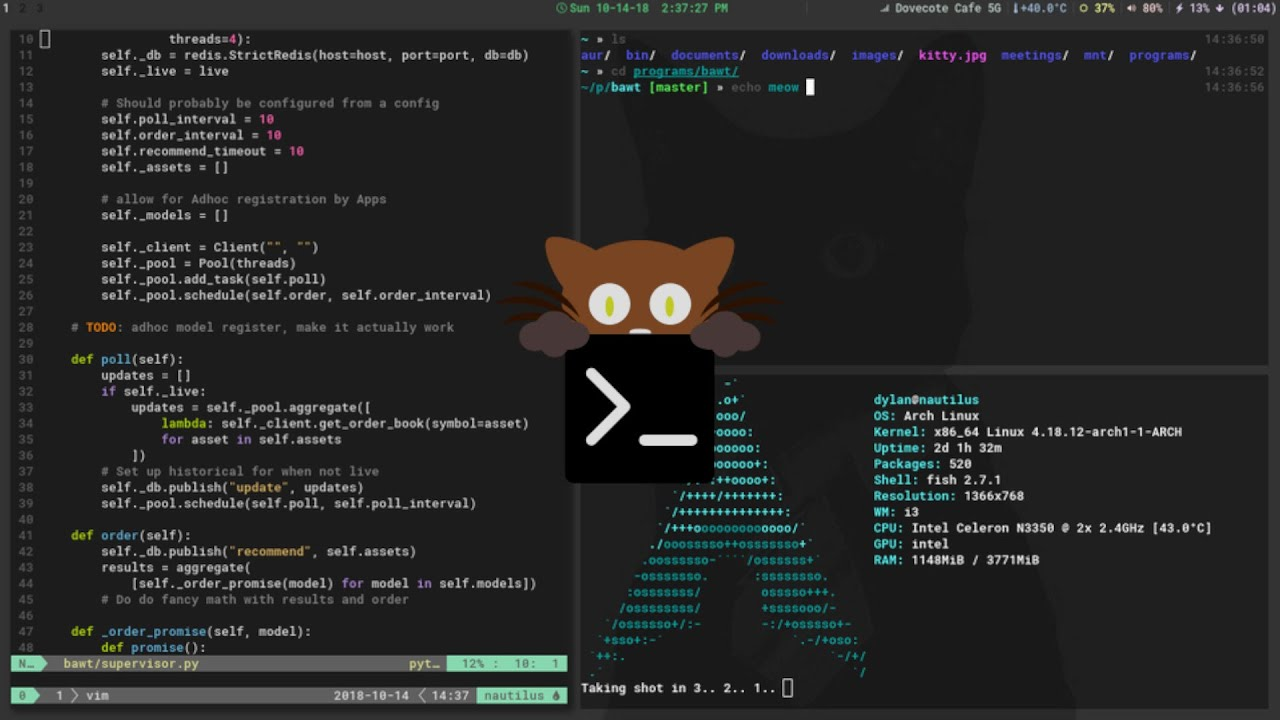
\includegraphics[width=0.9\textwidth]{img/kitty_terminal.jpg}
                \caption{\href{https://sw.kovidgoyal.net/kitty/}{Kitty}}
            \end{figure}
        \end{column}
        \begin{column}{0.5\textwidth}
            \begin{figure}
                \centering
                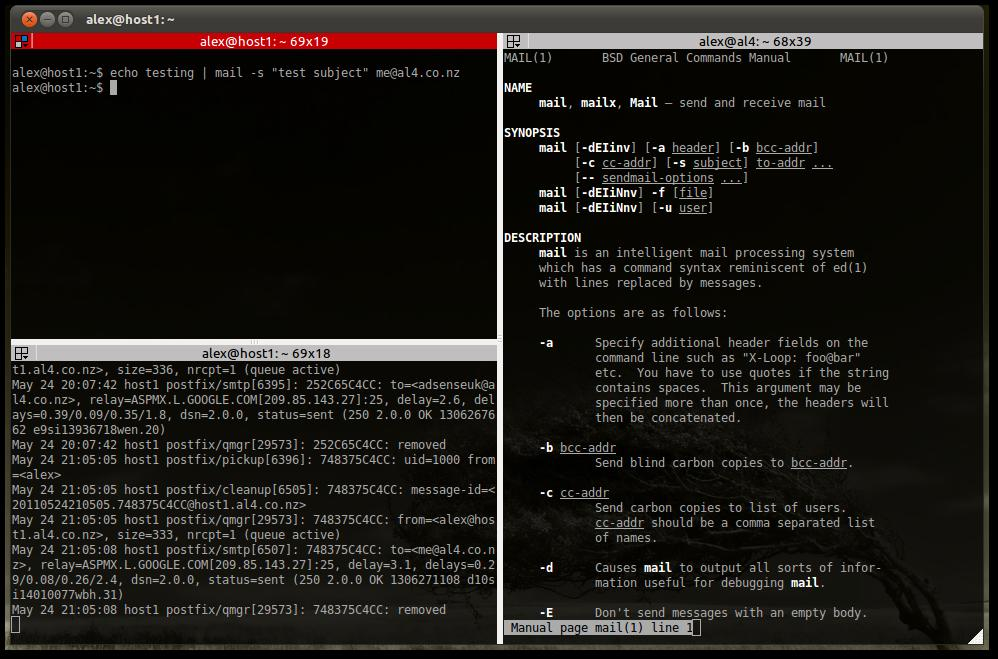
\includegraphics[width=0.9\textwidth]{img/terminator_terminal.jpg}
                \caption{\href{https://gnome-terminator.org/}{Terminator Terminal Emulator}}
            \end{figure}
        \end{column}
    \end{columns}

\end{frame}

\subsection{Shells}

\begin{frame}
    \frametitle{Shells}
    Existen distintos programas de terminal, con distintas funcionalidades (configuración, autocompletado, plugins, etc.).\\
    Son extremadamente fáciles de intercambiar (\href{https://man7.org/linux/man-pages/man1/chsh.1.html}{\texttt{chsh}}), y aún más rápido de arrancar una u otra (son programas: eg. \href{https://www.man7.org/linux/man-pages/man1/bash.1.html}{\texttt{bash}}). 

    % images
    \begin{columns}[c]
        \begin{column}{0.5\textwidth}
            \begin{figure}
                \centering
                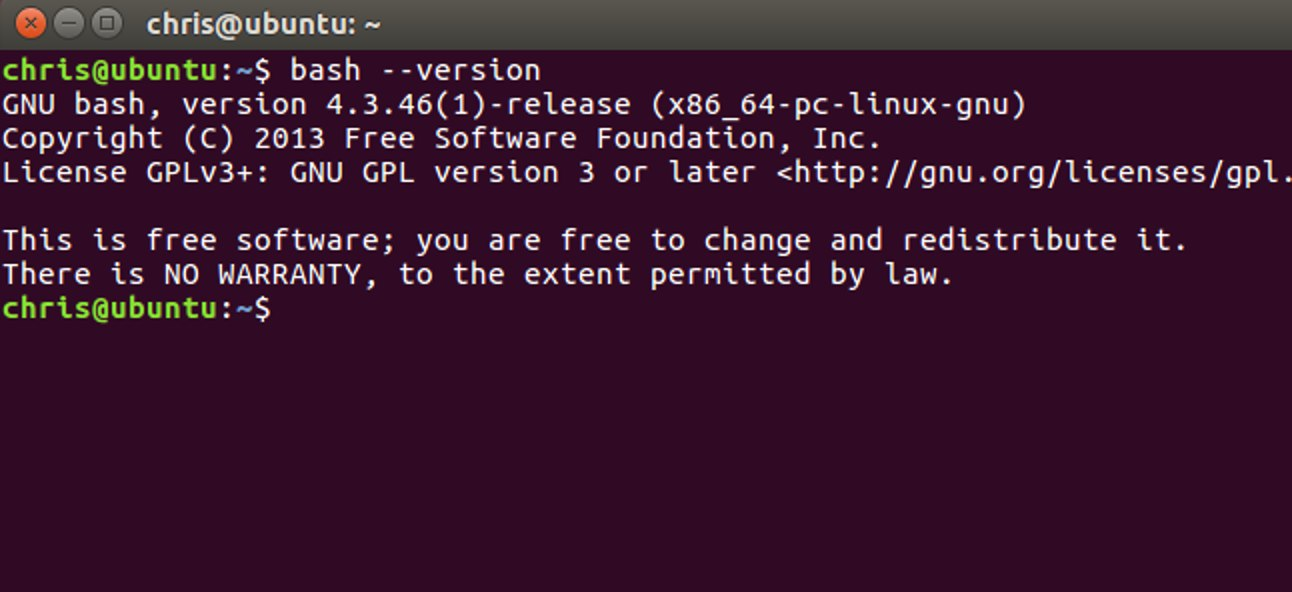
\includegraphics[width=0.9\textwidth]{img/bash_shell.jpg}
                \caption{Bash}
            \end{figure}
        \end{column}
        \begin{column}{0.5\textwidth}
            \begin{figure}
                \centering
                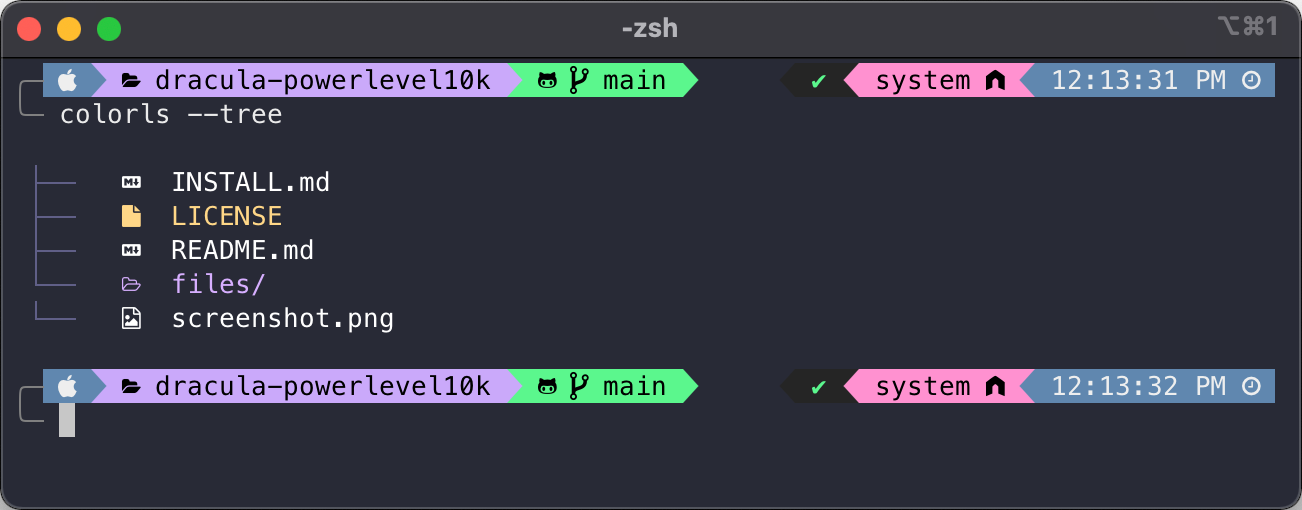
\includegraphics[width=0.9\textwidth]{img/powerlevel10k.png}
                \caption{\href{https://www.zsh.org/}{Z-Shell }\href{https://github.com/romkatv/powerlevel10k}{(con powerlevel10k)}}
            \end{figure}
        \end{column}
    \end{columns}

\end{frame}


\subsection{Dotfiles}

\begin{frame}
    \frametitle{Dotfiles}
    En Linux la mayoría de aplicaciones \textbf{guardan su configuración en archivos de texto plano}, ya sea en \texttt{/etc/} o en \texttt{/home/<user>}, y suelen llamarse "\texttt{.<program>rc}", de ahí su nombre de "\textit{resource files}" o "\textit{dotfiles}".\newline

    Ésto hace que crear, modificar, y compartir configuraciones sea muy sencillo y poderoso (\textit{scripting}, \href{https://github.com/rajayonin/dotfiles}{repositorios}, ...).

    \begin{figure}
        \centering
        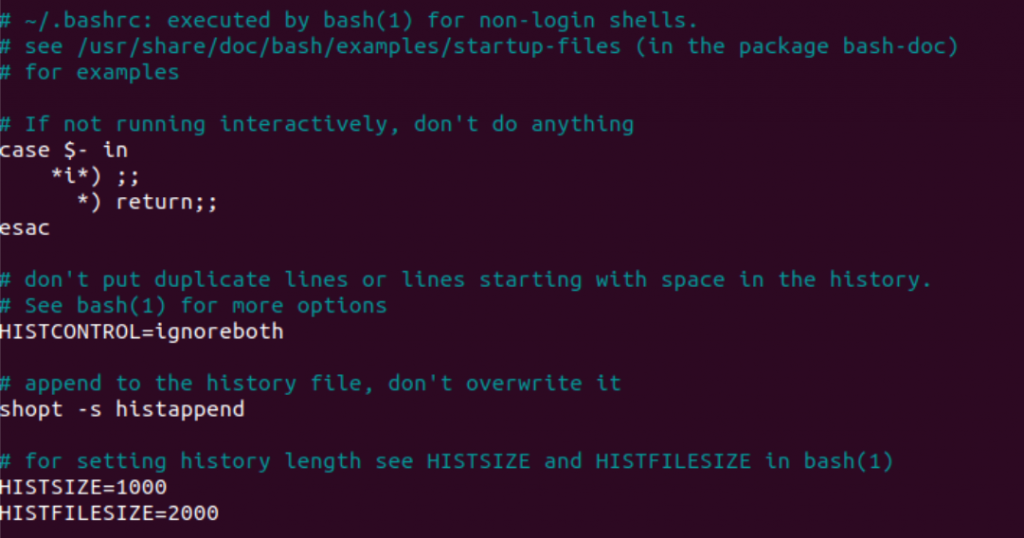
\includegraphics[width=0.4\textwidth]{img/bashrc.png}
        \caption{.bashrc}
    \end{figure}


\end{frame}


\section{La terminal}
% Sintaxis: flags, parámetros, y argumentos, prompt
% Funcionalidades de shell: |, >>, >, <, &&, contraseñas no se muestran en pantalla, Ctrl-L, Ctrl-C, Ctrl-D, Ctrl-Shift-C, Ctrl-Shift-V, Ctrl-R
% Gestión de procesos: nohup, &, Ctrl-z, fg, at
% Shell scripts
% Comandos (https://www.youtube.com/watch?v=s3ii48qYBxA, https://www.youtube.com/watch?v=PeCBpI1hT2Q&t=19s): 
% - Basic: ls, mv, cp, rm, cd, mkdir
% - Coreutils (https://www.maizure.org/projects/decoded-gnu-coreutils/): find, which/whereis, who, grep, echo, history, sudo, df/du, script, checksum
%   - Work w/ files: touch, cat, xxd, less, head, tail, sort, uniq, diff/comm, cmp, sed/awk, wc, cut, expand/unexpand, jq, yq, xmlint
% - Processes: top / ps, service, kill/kilall
% - Sesión: shutdown, reboot, logout
% - Network: ping, traceroute, ifconfig, wget, curl
% - File system: mount, fdisk/gparted, zip/unzip/tar
% - Other: lscpu, neofetch, tmux
% - Coña: cowsay, fortune, sl, cmatrix, lolcat, fortune | cowsay -f tux | lolcat (https://www.youtube.com/watch?v=iAdpkqLD4f0)
% Editores de texto en terminal: nano/micro, vim/nvim (lazyvim), emacs
% Reemplazos de comandos: trash, locate, htop, exa, bat
% Configurar terminal: aliases, PS1 (prompt)

\begin{frame}
    \frametitle{La terminal}
    La principal funcionalidad de la shell/TTY/terminal es ejecutar programas.\\
    Los programas más genéricos y usados para interactuar con el SO se suelen llamar "comandos".\newline

    Por defecto busca los programas en \texttt{/usr/bin/}, pero también puedes especificar el archivo con su \textit{path}\footnote{El archivo tiene que ser ejecutable.}.\newline

    Suele consistir de un \textit{prompt}, que indica el estado, y un cursor para escribir los comandos (ejecutados con el \texttt{Enter}).\\
    El prompt suele tener el formato \texttt{<user>@<host>:<cwd><\$\#>}, consistente del nombre del usuario, el nombre de la máquina (\textit{host}), el directorio actual (\textit{Current Working Directory}), y un caracter indicando el modo: \texttt{\$} para usuario y \texttt{\#} para superusuario.

\end{frame}


\begin{frame}
    \frametitle{Sintaxis general}
    
    La sintaxis general de cualquier comando es:\\
    \texttt{<cmd> [-<f>] [--<flag>] [<parameters>] [<arguments>]}\\
    Eg.: \texttt{tar -rvf ../stuff.tar --exclude-from exclude\_file .}

    \begin{itemize}
        \item \textbf{Flags:} Son opciones del comando. Dependiendo de la opción pueden implicar la presencia de un parámetro. Pueden ser escritas con una letra (\texttt{-<f>}) o una palabra (\texttt{--<flag>}), normalmente equivalentes (e.g: \texttt{-h} y \texttt{--help}). Normalmente puedes juntar varios \textit{flags} de una letra: \texttt{-<f><g><h>}.
        \item \textbf{Parámetros:} Expanden las opciones del comando.
        \item \textbf{Argumentos:} Los \textit{inputs} del comando. Suelen ser archivos.
    \end{itemize}
    

\end{frame}


\subsection{Funcionalidades de la terminal}

\begin{frame}
    \frametitle{Funcionalidades de la terminal (I)}
    La shell también trae una serie de funcionalidades extra:

    \begin{itemize}
        \item \textbf{Concatenaciones:} Sirven para concatenar comandos:\\
        \texttt{<cmd1> <cc> <cmd2>}\\
        \begin{itemize}
            \item \texttt{;} ejecuta \textbf{siempre} el segundo comando cuando termina el primero (THEN).
            \item \texttt{\&\&} ejecuta el segundo comando sólo \textbf{si el primero ha funcionado} (retorna \texttt{0}) (AND).
            \item \texttt{||} ejecuta el segundo sólo \textbf{si el primero ha fallado} (OR).
        \end{itemize}
        % E.g.: \texttt{sudo apt update \&\& apt upgrade}
        \item \textbf{Pipes:} Conectan la salida de un comando (\texttt{stdout}) a la entrada (\texttt{stdin}) del siguiente comando. \\
        Útil para enlazar comandos: \texttt{<cmd1> | <cmd2>}
        % Mítico ejemplo, buscar algo en un directorio: \texttt{ls | grep "algo"}.
        \item \textbf{Redirecciones:} Redirigen la entrada ó salida de un comando a un archivo: \texttt{<cmd> <rr> <file>}.
        \begin{itemize}
            \item \texttt{>} redirige la salida de un comando a un archivo (sobreescribe).
            \item \texttt{>>} concatena la salida de un comando a un archivo (no sobreescribe).
            \item \texttt{<} redirige los contenidos de un archivo a la entrada del comando.
        \end{itemize} 
        % E.g.: \texttt{cat a >> b}

    \end{itemize}

\end{frame}

\begin{frame}
    \frametitle{Funcionalidades de la terminal (II)}

    \begin{itemize}
        \item \textbf{Sudo:} Ejecuta el siguiente comando como \textit{root}: \texttt{sudo <cmd>}.
        \item \textbf{Contraseñas:} No se muestra \textit{nada} en pantalla (se puede cambiar en \texttt{/etc/sudoers} \footnote{Más info en \href{https://www.howtogeek.com/194010/how-to-make-password-asterisks-visible-in-the-terminal-window-in-linux/}{howtogeek.com/194010}.}). 
        \item \textbf{Copiar y pegar:} Se usan \texttt{Ctrl-Shift-C} y \texttt{Ctrl-Shift-V}.
        \item \textbf{Cancelar comandos:} Cancela el comando que estás ejecutando actualmente con \texttt{Ctrl-C}.
        \item \textbf{Cerrar sesión:} Cierra la sesión de terminal actual con \texttt{Ctrl-D} (útil para SSH).
        \item \textbf{Limpiar pantalla:} Con \texttt{Ctrl-L}, ó \texttt{clear}.
        \item \textbf{Borrar línea:} Borra el comando que estás escribiendo con \texttt{Ctrl-U}.
        \item \textbf{Autocompletado:} Con el \texttt{Tab}. Si hay más de una opción posible, tienes que darle dos veces\footnote{Como norma general, aunque depende de la shell.}.
    \end{itemize}

\end{frame}

\begin{frame}
    \frametitle{Funcionalidades de la terminal (III)}
    
    La mayoría de shells cuentan con un historial de comandos, normalmente guardado en \texttt{/home/<user>/.<shell>\_history} (eg. \texttt{.bash\_history})\footnote{También puedes ver el historial con \texttt{history}.}.\newline
    
    Viene con un tamaño máximo definido en la configuración de la shell, y se guarda entre sesiones del mismo usuario.
    \begin{itemize}
        \item Puedes navegar el historial con las flechas del teclado (arriba y abajo).
        \item Con \texttt{Ctrl-R} puedes hacer una búsqueda dentro historial. Sigue pulsando \texttt{Ctrl-R} para seguir buscando hacia atrás, y pulsa \texttt{Esc} para salir.
        \item Puedes repetir el último comando con \texttt{!!} y el comando \textit{n} veces anterior con \texttt{!-<n>}.
    \end{itemize}

\end{frame}


\subsection{Gestión de procesos}

\begin{frame}
    \frametitle{Gestión de procesos}
    
    Los procesos en Linux pueden estar en ejecutándose en \textit{foreground}, bloqueando la terminal actual, en \textit{background}, sin bloquearla \footnote{Un proceso en \textit{background} sigue pudiendo sacar mensajes por pantalla y, aunque puedas seguir usando la terminal, se vuelve difícil (prueba \texttt{ping 8.8.8.8 \&}).}; o en suspensión, parado y quietecito.

    \begin{itemize}
        \item Puedes lanzar un proceso en \textit{background} con \texttt{<cmd> \&}. 
        \item Para suspender un proceso ejecutándose en \textit{foreground}, usa \texttt{Ctrl-Z}.
    \end{itemize}
    
    Ambos retornarán un número de proceso en background, e.g \texttt{[1]}.
    
    \begin{itemize}
        \item Para traer al \textit{foreground} el proceso \textit{n}\footnote{Procesos tanto en \textit{background} como en suspensión.} basta con usar \texttt{\%<n>}\footnote{Equivalente a \texttt{fg <n>}.}. Para el último proceso, basta con usar \texttt{\%}.
        \item Para evitar que un proceso termine cuando se cierra la sesión, usa \texttt{nohup <cmd>} (recomendable usar junto con \texttt{\&}).
        \item Puedes programar la ejecución de un comando (o shell script) con \texttt{at <time> <cmd>}.
    \end{itemize}

\end{frame}


\subsection{Shell scripts}

\begin{frame}
    \frametitle{Shell scripts}
    
    Linux te permite crear \textit{scripts} para terminal, muy útiles para hacer tareas repetitivas, y en general para la automatización\footnote{También recomiendo automatizar con \href{https://www.gnu.org/software/make/manual/make.html}{GNU make}.}.\\
    Cuentan con un "lenguaje de programación" propio, con variables, funciones, sentencias de control, y comentarios; aparte de todas las funcionalidades de la terminal.\newline

    El "lenguaje" más usado es Bash Script.
    \begin{itemize}
        \item Se suelen guardar con la extensión \texttt{.sh} y en la primera línea se suele poner \texttt{\#!/bin/bash}.
        \item Cada línea se trata como un comando y se ejecuta en la terminal actual.
        \item Los comentarios usan \texttt{\#}.
        \item Es recomendable ejecutarlos con \texttt{bash <script.sh>}, aunque se pueden ejecutar el archivo directamente (\texttt{<script.sh>}\footnote{Recuerda que hay que especificar el \textit{path} completo, eg. \texttt{./<script.sh>}.}).
    \end{itemize}

\end{frame}


\subsection{Comandos}

\begin{frame}
    \frametitle{Comandos: Básicos}
    Los comandos básicos son:

    \begin{itemize}
        \item \texttt{ls}: Muestra los contenidos del directorio (\texttt{-lah} para mostrar toda la info).
        \item \texttt{cd <dir>}: Moverse al directorio \texttt{dir}.
        \item \texttt{mv <origin> <destination>}: Mover archivo \texttt{origin} al \textit{path} \texttt{destination} (\texttt{-r} para carpetas).
        \item \texttt{cp <origin> <destination>}: Mover archivo \texttt{origin} al \textit{path} \texttt{destination} (\texttt{-r} para carpetas).
        \item \texttt{rm <file>}: Eliminar el archivo \texttt{file} (\texttt{-r} para carpetas).
        \item \texttt{mkdir <dir>}: Crea el directorio \texttt{dir}.
    \end{itemize}
\end{frame}

\begin{frame}
    \frametitle{Comandos: Generales\footnote{Echadle un vistazo a las \href{https://www.maizure.org/projects/decoded-gnu-coreutils/}{\textit{coreutils}}.}}

    \begin{itemize}
        \item \texttt{who}: Muestra los usuarios \textit{loggeados} actualmente en el \textit{host}.
        \item \texttt{echo <msg>}: Imprime texto por pantalla.
        \item \texttt{find <dir> -iname <file>}: Busca archivos en un directorio (y subdirectorios).
        \item \texttt{which <cmd>}\footnote{\texttt{whereis} da más información, pero es más lento.}: Busca el \textit{path} donde está guardado un ejecutable.
        \item \texttt{script}: \textit{Loggea} la terminal y lo guarda en un archivo (usa \texttt{exit} para parar).
        \item \texttt{df -h}: Muestra información del espacio usado en disco.
        \item \texttt{du -h <dir>}: Muestra información del espacio usado en un directorio (y subdirectorios).
        \item \texttt{cksum <file>}: Calcula el \textit{checksum} de un archivo.
        \item \texttt{grep <str> <file>}: Busca patrones en archivos. También útil con \textit{pipes} para buscar en \textit{outputs} de comandos: \texttt{<cmd> | grep <str>}.
    \end{itemize}
\end{frame}

\begin{frame}
    \frametitle{Comandos: Trabajando con archivos (I)}

    \begin{itemize}
        \item \texttt{touch <file>}: Crea un archivo vacío.
        \item \texttt{cat <file>}: Imprime por pantalla los contenidos de un archivo.
        \item \texttt{xxd <file>}: Muestra el archivo en hexadecimal.
        \item \texttt{wc <file>}: Muestra el número de líneas, palabras, y bytes de un archivo.
        \item \texttt{less <file>}: Visor de archivos con funcionalidades extra (mejor que \texttt{cat} para archivos grandes). Pulsa \texttt{q} para salir.
        \item \texttt{head <file>}: Muestra las primeras líneas de un archivo (\texttt{head -n <n> <file>} para mostrar \textit{n} líneas).
        \item \texttt{tail <file>}: Muestra las últimas líneas de un archivo (\texttt{tail -n <n> <file>} para mostrar \textit{n} líneas).
        \item \texttt{sort <file>}: Ordena el archivo alfanuméricamente y lo saca por pantalla.
        \item \texttt{uniq <file>}: Elimina las líneas repetidas de un archivo y lo saca por pantalla.
    \end{itemize}
\end{frame}

\begin{frame}
    \frametitle{Comandos: Trabajando con archivos (II)}

    \begin{itemize}
        \item \texttt{tac\footnote{"tac" es "cat" al revés.} <file>}: Da la vuelta a un archivo (línea a línea) y lo saca por pantalla (\texttt{rev} para byte a byte).
        \item \texttt{diff\footnote{\texttt{comm} es similar pero más flexible.} <file1> <file2>}: Muestra las diferencias entre dos archivos.
        \item \texttt{cmp <file1> <file2>}: Comprueba si dos archivos son iguales.
        \item \texttt{cut -c <n>- <file>}: Corta los \textit{n} primeros caracteres de cada línea (\texttt{-<n>} para los \textit{n} últimos).
        \item \texttt{expand <file>}: Convierte \textit{tabs} a espacios.
        \item \texttt{unexpand <file>}: Convierte espacios a \textit{tabs}.
        \item \texttt{sed}/\texttt{awk}: Permiten editar archivos desde comandos. Muy poderosos para \textit{scripting} (especialmente \texttt{awk}).
        \item \texttt{jq}/\texttt{yq}/\texttt{xmlint}: Similares a \texttt{sed}, pero para formatos específicos: JSON, yaml, XML...
    \end{itemize}
\end{frame}


\begin{frame}
    \frametitle{Comandos: Procesos y sesiones}

    \begin{itemize}
        \item \texttt{ps}: Muestra los procesos activos.
        \item \texttt{top}\footnote{El Administrador de tareas de terminal.}: Muestra información de procesos y recursos en tiempo real.
        \item \texttt{service <service>\footnote{Los servicios son los scripts que están en \texttt{/etc/init.d/}.} stop}: Para un servicio en ejecución. También puedes ver su estado (\texttt{status}) o reiniciarlo (\texttt{restart}).
        \item \texttt{kill <pid>}: Mata a un proceso dado su PID (Process ID) (\texttt{-9} para forzar la muerte).
        \item \texttt{killall <name>}: Mata todos los procesos asociados a un nombre.
    \end{itemize}
    \vspace{8pt}
    \begin{itemize}
        \item \texttt{shutdown now}: Apaga el ordenador.
        \item \texttt{restart now}: Reinicia el ordenador.
        \item \texttt{logout}: Cierra la sesión (equivalente a \texttt{Ctrl-D}).
    \end{itemize}

\end{frame}


\begin{frame}
    \frametitle{Comandos: Network}

    \begin{itemize}
        \item \texttt{ping <dir>\footnote{Puedes especificar la dirección IP (eg. \texttt{8.8.8.8}) o un \textit{hostname} (eg. \texttt{google.com}).}}: Hace \textit{pings} contínuos a la dirección indicada.
        \item \texttt{traceroute <dir>}: Muestra la ruta hasta la dirección indicada.
        \item \texttt{wget <dir>}: Obtiene los archivos de una dirección web (HTTP/HTTPS y FTP).
        \item \texttt{curl}: Herramienta que permite enviar y recibir \textit{requests}, archivos, etc. Soporta muchos protocolos.
        \item \texttt{ifconfig}: Muestra la configuración de red. Éste comando también permite modificar la configuración.
    \end{itemize}

\end{frame}

\begin{frame}
    \frametitle{Comandos: Sistema de ficheros}

    \begin{itemize}
        \item \texttt{lsblk}: Muestra los discos y particiones del sistema (\texttt{-f} para ver más info como el UUID).
        \item \texttt{mount <partition>\footnote{Normalmente se encuentran en \texttt{/dev/}, eg. \texttt{/dev/sda}.} <path>}: Monta la partición en el directorio indicado\footnote{Para montar de forma permanente, hay que modificar \texttt{/etc/fstab}.}.
        \item \texttt{umount <partition>}: Desmonta la partición. 
        \item \texttt{fdisk}\footnote{Una alternativa gráfica es \texttt{gparted}.}: Utilidad para administrar las particiones del disco.
    \end{itemize}

\end{frame}

\begin{frame}
    \frametitle{Comandos: Archivos comprimidos}

    \begin{itemize}
        \item \texttt{zip <archive.zip> <files>}: Comprime los archivos. Usa \texttt{-r} para directorios, y \texttt{-x <files>} para excluir archivos.
        \item  \texttt{unzip <archive.zip> [-d <path>]}: Descomprime el archivo al \textit{path} especificado (por defecto, el actual).
        \item  \texttt{tar -tvf <archive.tar>}: Lista los contenidos del archivo comprimido.
        \item \texttt{tar -cvf <archive.tar> <files>}: Usa \texttt{-r} para directorios, y \texttt{--exclude-from <exclude-file>} para excluir los archivos definidos en el \textit{exclude file}. Para comprimir Tar Gz, usa \texttt{-z}.
        \item \texttt{tar -xvf <archive.tar> [-C <path>]}: Descomprime el archivo al \textit{path} especificado (por defecto, el actual). También puedes descomprimir archivos específicos: \texttt{tar -xvf <archive.tar> <files>}.
    \end{itemize}

\end{frame}

\begin{frame}
    \frametitle{Comandos: Otros}

    \begin{itemize}
        \item \texttt{lscpu}: Muestra información de la CPU.
        \item \texttt{neofetch\footnote{\href{https://github.com/dylanaraps/neofetch}{github.com/dylanaraps/neofetch}}}: Muestra información del sistema.
        \item \texttt{tmux\footnote{\href{https://github.com/tmux/tmux}{github.com/tmux/tmux}}}: Multiplexador de terminal. Permite tener varias "ventanas" en la misma terminal.
        \item \texttt{tree [-L <n>] <dir>}: Muestra un diagrama de árbol de todos los archivos y subdirectorios del directorio especificado, con nivel de profundidad máximo \textit{n}.
    \end{itemize}

\end{frame}

\begin{frame}
    \frametitle{Comandos: Comandos chorra}
    Porque no todo debe ser útil.

    \begin{itemize}
        \item \texttt{cowsay <msg>}: Muestra el mensaje como si lo dijera una vaca.
        \item \texttt{fortune}: Una fuente casi infinita de sabiduría.
        \item \texttt{sl}: Animación de un trenecito que se activa cada vez que escribes \texttt{ls} mal.
        \item \texttt{lolcat}: Un \texttt{cat} arcoíris.
        \item \texttt{bastet}: El Tetris bien hecho.
        \item \texttt{cmatrix -a}: Conviértete en hacker.
        \item \texttt{:()\{:|:\&\};:}: Fork bomb.
        \item \texttt{rm -fr /}: Elimina el idioma francés del sistema\footnote{Obviamente no hace eso.}.
    \end{itemize}

\end{frame}

\begin{frame}
    \frametitle{Comandos: Comandos chorra}
    \begin{figure}
        \centering
        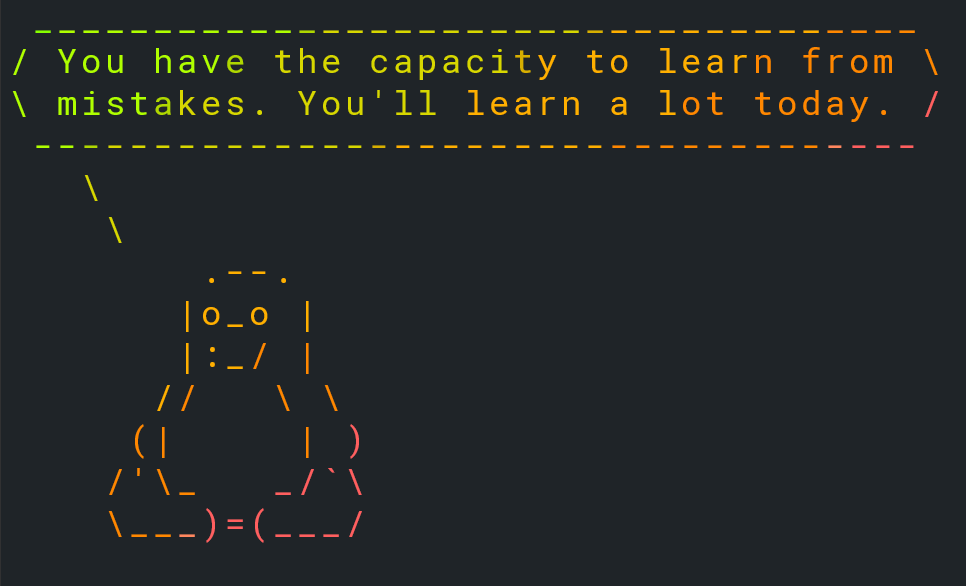
\includegraphics[width=0.6\textwidth]{img/wisdom.png}
        \caption{\texttt{fortune | cowsay -f tux | lolcat}}
    \end{figure}
\end{frame}

\begin{frame}
    \frametitle{Mejores comandos}
    La comunidad FOSS y Linux crea reemplazos para los comandos clásicos que mejoran sus funcionalidades.\newline

    Algunos ejemplos son \texttt{trash}\footnote{\href{https://github.com/andreafrancia/trash-cli}{github.com/andreafrancia/trash-cli}} (\texttt{rm}), \texttt{locate}\footnote{Parte de \href{https://pagure.io/mlocate}{mlocate}.} (\texttt{find}), \texttt{btop}\footnote{\href{https://github.com/aristocratos/btop}{github.com/aristocratos/btop}} (\texttt{top}), \texttt{exa}\footnote{\href{https://github.com/ogham/exa}{github.com/ogham/exa}} (\texttt{ls}), o \texttt{bat}\footnote{\href{https://github.com/sharkdp/bat}{github.com/sharkdp/bat}} (\texttt{cat}).

    % images
    \begin{columns}[c]
        \begin{column}{0.4\textwidth}
            \begin{figure}
                \centering
                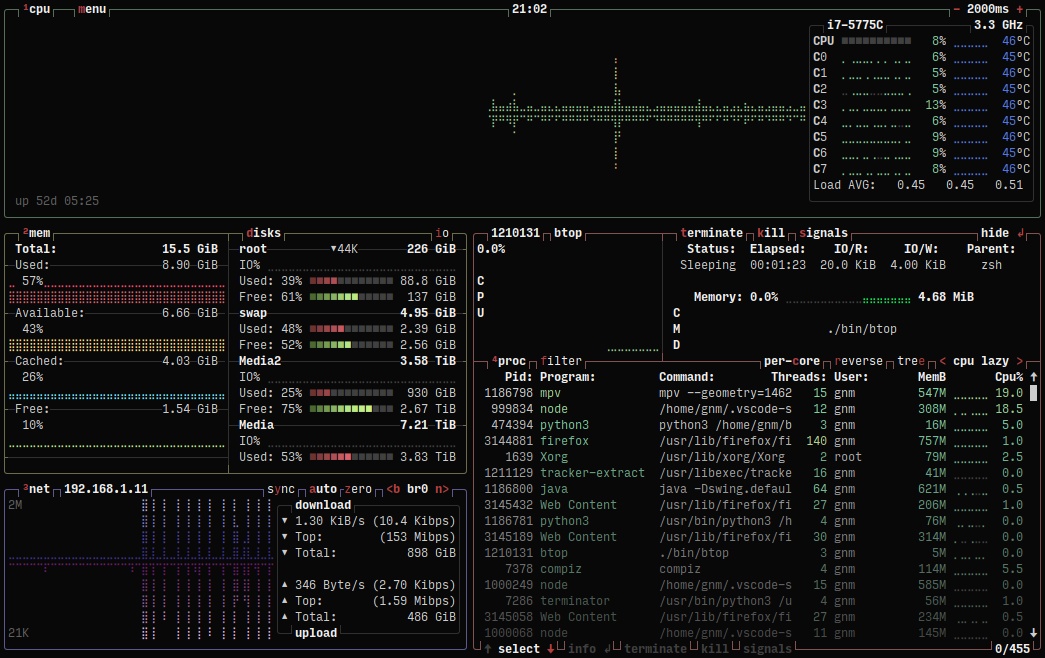
\includegraphics[width=0.9\textwidth]{img/btop.png}
                \caption{\href{https://github.com/aristocratos/btop}{btop}}
            \end{figure}
        \end{column}
        \begin{column}{0.4\textwidth}
            \begin{figure}
                \centering
                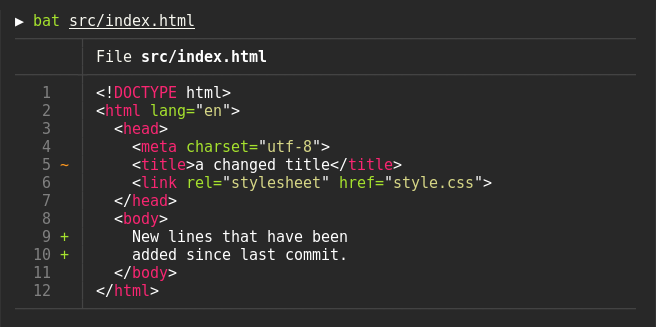
\includegraphics[width=0.9\textwidth]{img/bat.png}
                \caption{\href{https://github.com/sharkdp/bat}{bat}}
            \end{figure}
        \end{column}
    \end{columns}
\end{frame}


\subsection{Editores de texto en terminal}

\begin{frame}
    \frametitle{Editores de texto en terminal}
    Muy útiles cuando no dispones de GUI o para ver y modificar archivos rápidamente desde la propia terminal.\newline

    Tienden a ser mucho más eficientes en el uso de recursos, y a proporcionar muchas más funcionalidades, personalización, y lenguajes de \textit{scripting}.\\
    Van desde los más simples e intuitivos (nano o micro\footnote{\href{https://github.com/zyedidia/micro}{github.com/zyedidia/micro}}), a los más avanzados (vim/neovim\footnote{Recomiendo \href{https://www.lazyvim.org/}{LazyVim}.} o emacs).

    % images
    \begin{columns}[c]
        \begin{column}{0.4\textwidth}
            \begin{figure}
                \centering
                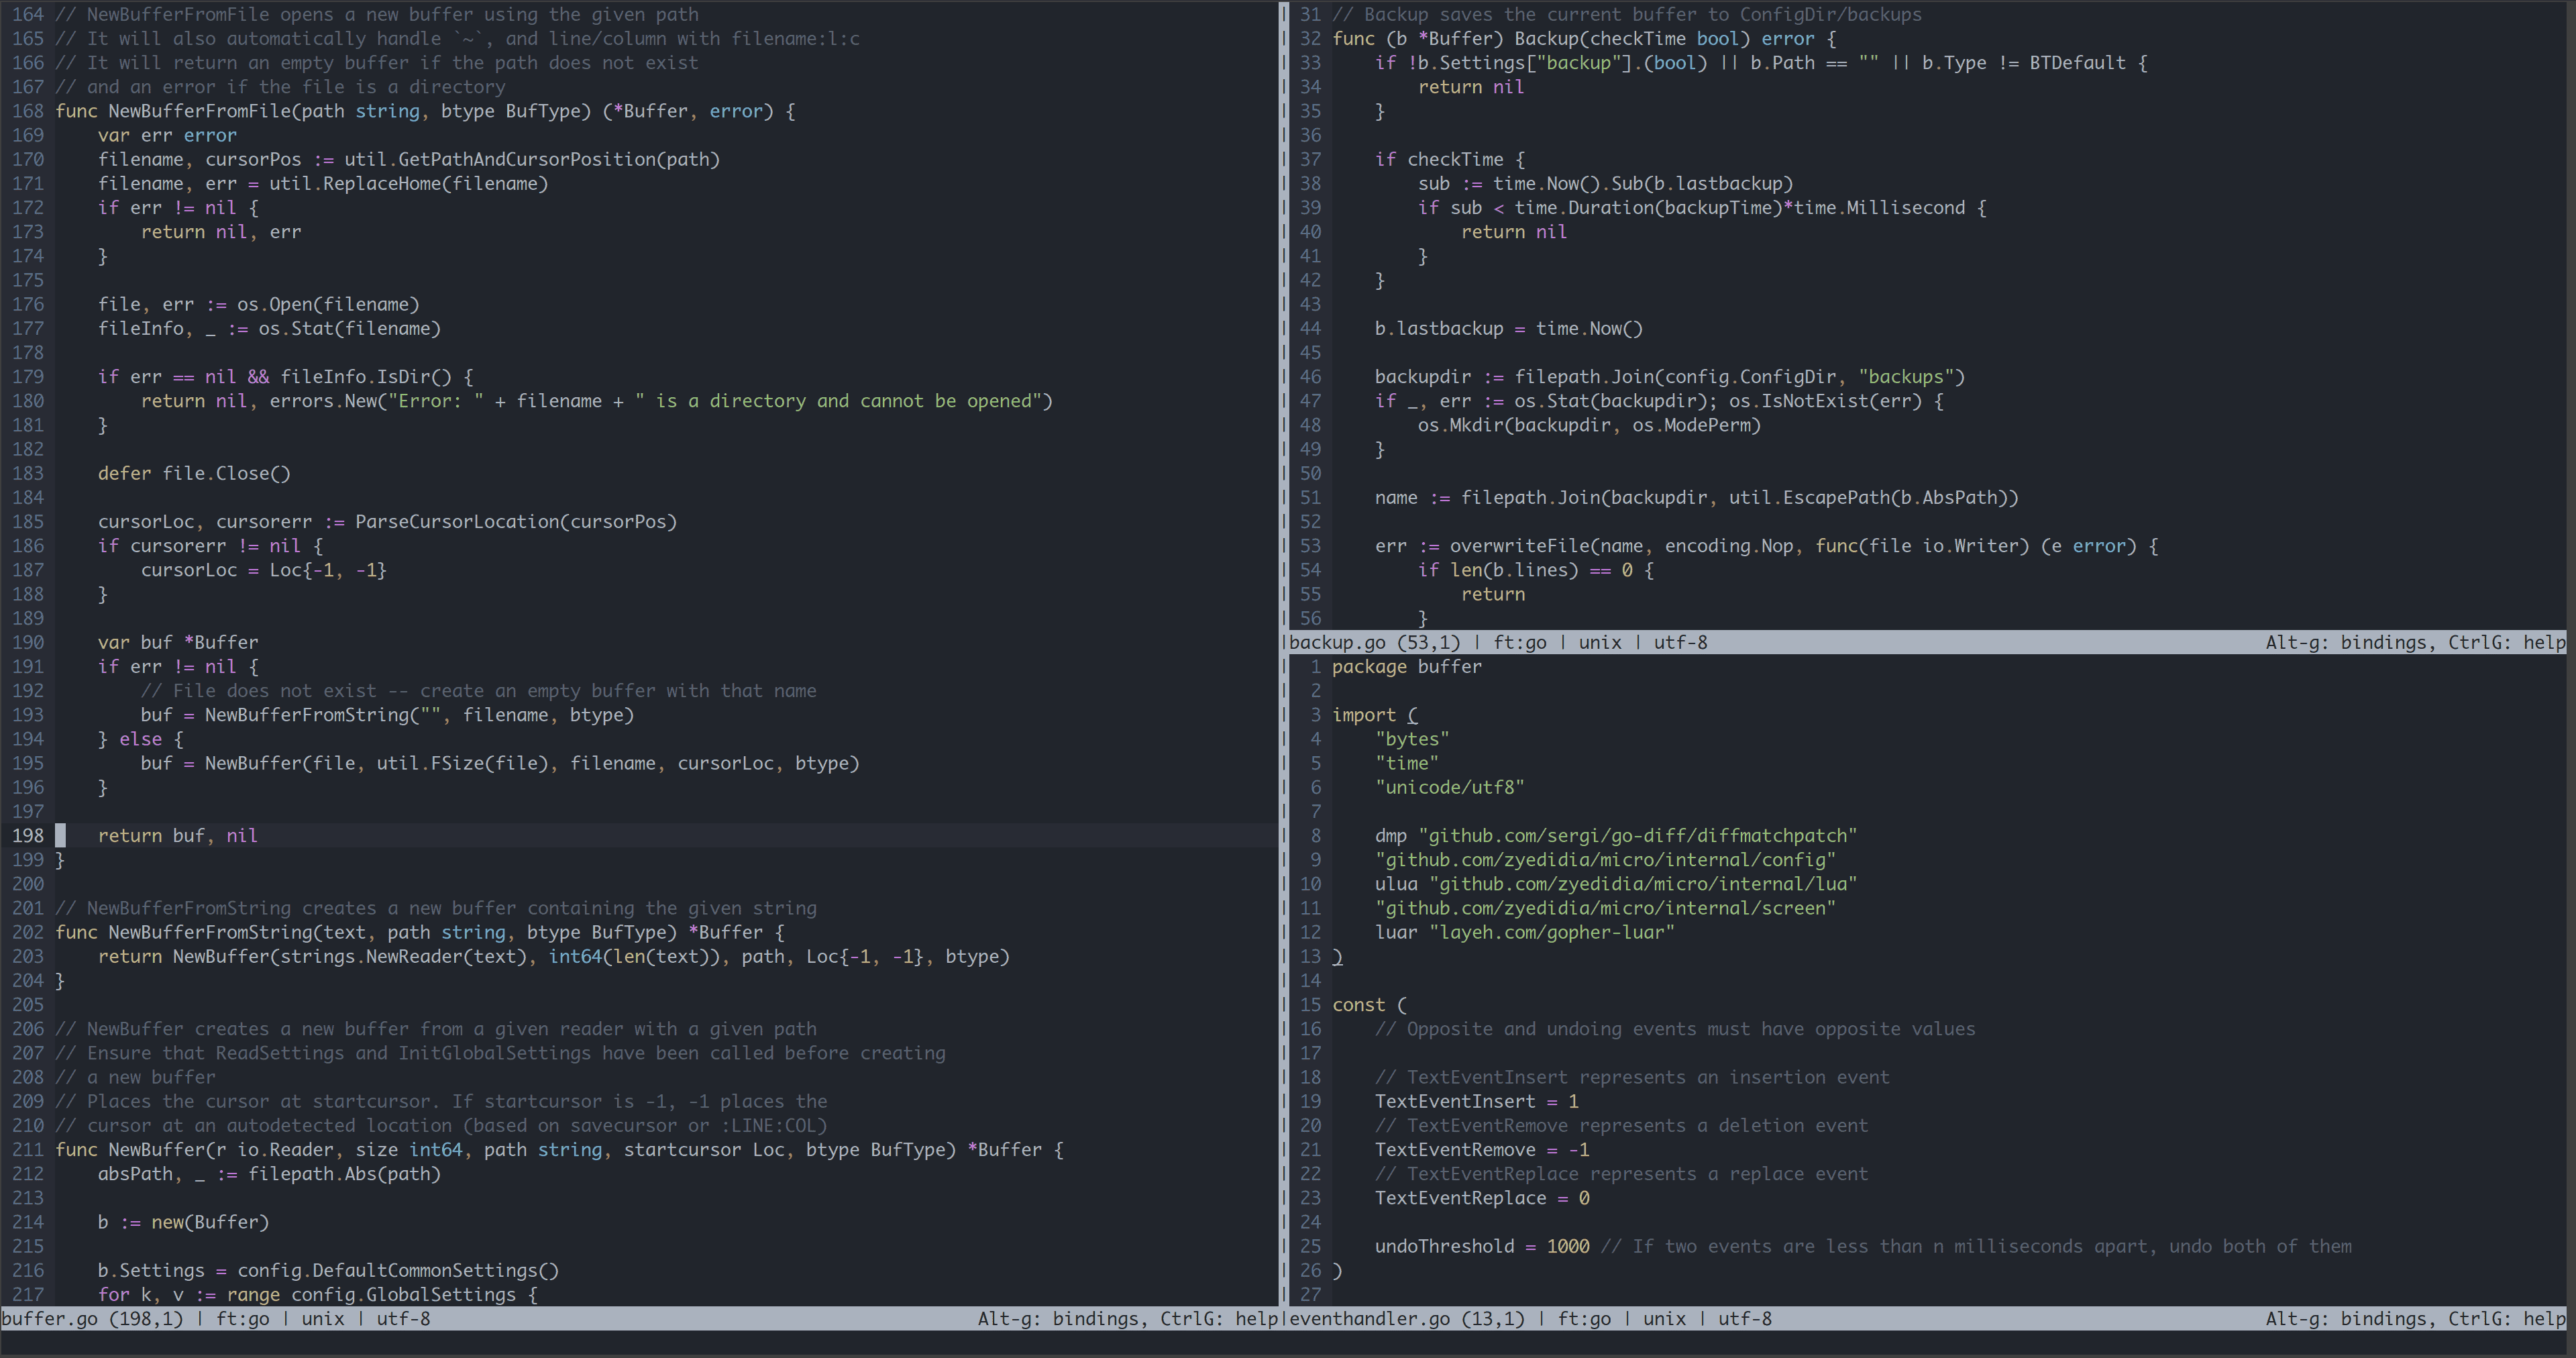
\includegraphics[width=0.9\textwidth]{img/micro.png}
                \caption{\href{https://github.com/zyedidia/micro}{Micro}}
            \end{figure}
        \end{column}
        \begin{column}{0.4\textwidth}
            \begin{figure}
                \centering
                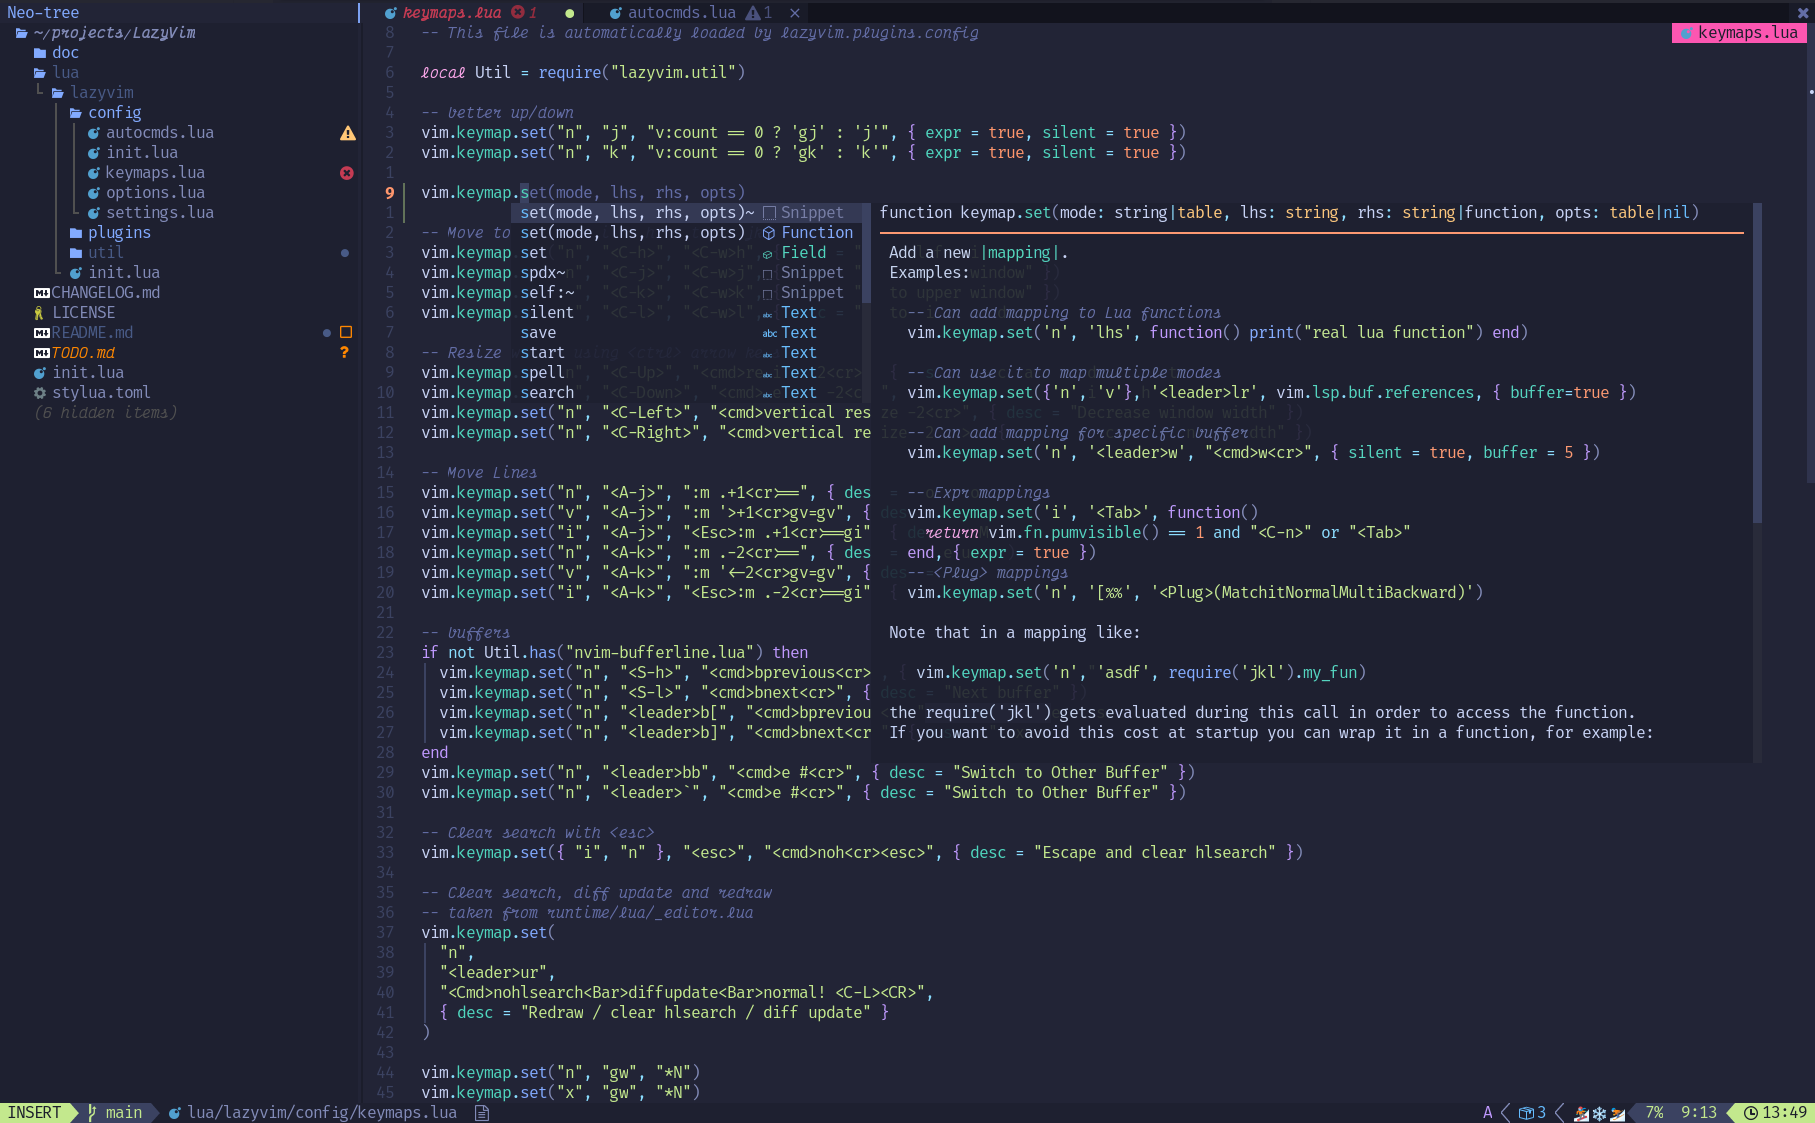
\includegraphics[width=0.8\textwidth]{img/lazyvim.png}
                \caption{\href{https://neovim.io/}{Neovim} con \href{https://www.lazyvim.org/}{LazyVim}}
            \end{figure}
        \end{column}
    \end{columns}

\end{frame}




\subsection{Personalizando la terminal}

\begin{frame}
    \frametitle{Personalizando la terminal}
    Dependiendo de la shell, habrá más o menos configuraciones, pero las básicas son:

    \begin{itemize}
        \item \textbf{Alias:} Puedes crear alias (distintos nombres) para comandos, ya sea para acortar el nombre, o cambiarlo, o crear diferentes comandos nuevos. Ten en cuenta que un alias puede contener parámetros, o varios comandos concatenados, y pueden sobreescribirse unos a otros.\\
        Puedes crear alias permanentes añadiendo \texttt{alias <alias>="<cmd>"} al archivo de configuración de la shell (eg. \texttt{.bashrc}). Puedes ver todos los alias activos con \texttt{alias}.\\
        Para evitar que un comando ejecute un alias, usa \texttt{\textbackslash<cmd>}.\\
        \item \textbf{Prompt:} Es totalmente personalizable, normalmente se guarda en la variable \texttt{PS1} del archivo de configuración de la shell.
        \item \textbf{Startup:} Puedes ejecutar comandos al arrancar la terminal añadiéndolos directamente en el archivo de configuración de la shell.
    \end{itemize}

\end{frame}



\section{Permisos}
% rwx, chmod, etc.

\begin{frame}
    \frametitle{Permisos (I)}
    Linux implementa el control de acceso a archivos y directorios mediante el sistema UGO (User, Group, Other), y cada archivo o directorio pertenece a un usuario y a un grupo.\\
    Cada una de éstas entidades puede tener los siguientes permisos sobre el archivo/directorio:
    \begin{itemize}
        \item \texttt{r} - \textit{read}: Permite ver el archivo en el directorio y leer sus contenidos. En el caso de directorios, permite ver sus contenidos.
        \item \texttt{w} - \textit{write}: Permite modificar y eliminar el archivo. En el caso de directorios, permite crear y eliminar archivos.
        \item \texttt{x} - \textit{execute}: Permite ejecutar el archivo. En el caso de directorios, permite entrar en él.
    \end{itemize}

\end{frame}


\begin{frame}
    \frametitle{Permisos(II)}
    Con \texttt{ls -l} puedes ver los permisos de los archivos, entre otras cosas.\newline

    Los permisos tienen el formato \texttt{<d><rwx><rwx><rwx> <owner> <group>}, donde el primer caracter indica si es un archivo o un directorio (\texttt{d}), los tres siguientes indican los permisos del propietario (U), luego los del grupo (G), y finalmente los del resto de usuarios (O).\\
    Un guión (\texttt{-}) indica que ese permiso no está concedido.\newline

    Puedes añadir y quitar permisos con \texttt{chmod [<ugo>]<+-><rwx>[, ...] <file/dir>}, eg. \texttt{chmod u+x,-rw file}, o usando el modelo octal\footnote{Ejemplo en \href{https://www.multacom.com/faq/password_protection/file_permissions.htm}{multacom.com/faq/password\_protection/file\_permissions.htm}.}.

\end{frame}


\section{Más paquetes}
% Más gestores de paquetes: flatpak, snapd (malo), nix, nala (pa debian) 
% Appimage
% ¡Compila!
% LSW ("Linux Subsystem for Windows"): wine, Lutris, heroic games, steam (proton)

\begin{frame}
    \frametitle{Más paquetes}
    Algunos gestores de paquetes tienen falta de paquetes o paquetes desactualizados, por lo que a veces es necesario usar alternativas:

    \begin{itemize}
        \item \textbf{Gestores de paquetes alternativos:} Suelen tener las versiones más actualizadas de los paquetes, y son agnósticos. El problema suele ser el rendimiento. Los más usados son snapd\footnote{Bastante basura, pero aquí lo tienes: \href{https://snapcraft.io/}{snapcraft.io}.}, flatpak\footnote{\href{https://flatpak.org/}{flatpak.org}}, y Nix\footnote{\href{https://nixos.org/}{nixos.org}}.
        \item \textbf{Appimages\footnote{\href{https://appimage.org/}{appimage.org}}:} Ejecutables autocontenidos (\texttt{.Appimage}) que corren sobre cualquier Linux*, ...pero no se actualizan. 
        \item \textbf{Compilar:} Siempre puedes compilar tus propios programas desde el código fuente, si es FOSS...
    \end{itemize}

    También existen \textit{wrappers} (interfaces) para gestores de paquetes, recomiendo encarecidamente Nala\footnote{\href{https://gitlab.com/volian/nala}{gitlab.com/volian/nala}} para APT.

\end{frame}

\subsection{Linux Subsystem for Windows}
\begin{frame}
    \frametitle{LSW (Linux Subsystem for Windows)\footnote{Sí, me he inventado el término.}}
    Aunque parezca increíble, es posible ejecutar programas de Windows en Linux:
    
    \begin{itemize}
        \item \textbf{Wine\footnote{\href{https://www.winehq.org/}{winehq.org}}:} Capa de compatibilidad, permitiendo ejecutar (ciertos) programas de Windows en Linux.
        \item \textbf{Lutris\footnote{\href{https://lutris.net/}{lutris.net}}:} Plataforma (llevada por la comunidad) para instalar y ejecutar videojuegos en Linux.
        \item \textbf{Proton (Steam\footnote{\href{https://store.steampowered.com/}{store.steampowered.com}}):} Steam trae incorporado Proton, un \textit{fork} de Wine enfocado a videojuegos\footnote{Lista de juegos compatibles en \href{https://www.protondb.com/}{protondb.com}.}.
        \item \textbf{Heroic Games Launcher\footnote{\href{https://heroicgameslauncher.com/}{heroicgameslauncher.com}}:} \textit{Launcher} de Epic Games y GOG para Linux (incorpora Wine).
    \end{itemize}

\end{frame}


\section{Ayuda}
% man, -h/--help, whatis, tldr (https://tldr.sh/)

\begin{frame}
    \frametitle{Ayuda}
    Hay diferentes formas de obtener ayuda en Linux, sin tirar de Google (o DuckDuckGo):

    \begin{itemize}
        \item \textbf{Manual:} Cada programa instalado trae consigo una página del manual explicando T-O-D-O. Aparte de eso, el manual de Linux trae información sobre el propio Linux (configuración, etc.) y sobre el lenguaje de programación C.\\
        Basta con usar \texttt{man <término>}.
        \item \texttt{--help}: La mayoría de comandos y programas tienen un \textit{flag} de ayuda, donde explican brevemente el uso, la sintaxis y las distintas opciones y parámetros.
        \item \texttt{whatis <cmd>}: Muestra en una línea lo que hace el comando.
        \item \textbf{tldr pages\footnote{\href{https://tldr.sh/}{tldr.sh}}:} Páginas de manual más simples y hechas por la comunidad.
    \end{itemize}
\end{frame}


\section{Secure Shell Hashing}
% ssh, scp


\begin{frame}
    \frametitle{SSH (Secure Shell Hashing)}
    Permite conectarte a un ordenador a través de una terminal remota, o mover archivos, todo de forma segura.

    \begin{itemize}
        \item Para conectarse basta con usar \texttt{ssh <user>@<host>}.
        \item Para enviar un archivo usa \texttt{scp <file> <user>@<host>:<path>}.
        \item Para descargar un archivo usa \texttt{scp <user>@<host>:<file> <path>}.
    \end{itemize}

    Infinitamente usado para acceder a servidores\footnote{El Laboratorio del Departamento de Informática de la UC3M proporciona \href{https://www.lab.inf.uc3m.es/wp-content/docs/Manual_ConexionSSH.pdf}{Guernika}: \texttt{ssh a0<NIA-sin-el-100>@guernika.lab.inf.uc3m.es}.}, ya que normalmente no cuentan con GUI.

\end{frame}



\section{Backups}
% rclone: https://www.howtogeek.com/451262/how-to-use-rclone-to-back-up-to-google-drive-on-linux/

\begin{frame}
    \frametitle{Backups}
    
    Hacer copias de seguridad de datos en Linux es relativamente sencillo.\newline

    Quitando Git\footnote{Tutorial aquí: \href{https://www.youtube.com/watch?v=jvsneGS00Tw}{youtube.com/watch?v=jvsneGS00Tw}.}, Rclone\footnote{\href{https://rclone.org/}{rclone.org}} te permite hacerlo muy fácilmente e incluso sincronizarlo con Google Drive\footnote{\href{https://www.howtogeek.com/451262/how-to-use-rclone-to-back-up-to-google-drive-on-linux/}{howtogeek.com/451262}}.

    \begin{figure}
        \centering
        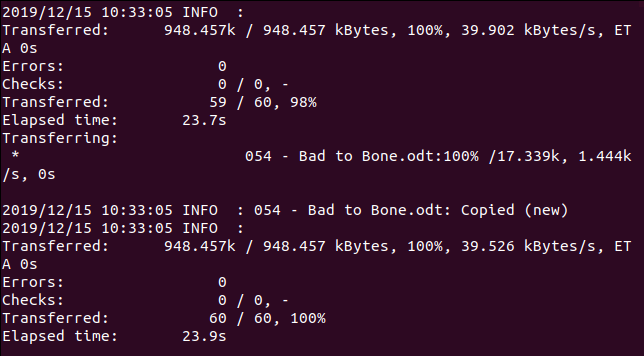
\includegraphics[width=0.5\textwidth]{img/rclone.png}
        \caption{\href{https://rclone.org/}{Rclone}}
    \end{figure}
\end{frame}



\begin{frame}
    \frametitle{¿Preguntas, reclamos, improperios?}
    \centering
    
\includegraphics[width=0.9\textwidth]{img/noot.png}
\end{frame}



\begin{frame}
    \frametitle{Más información}

    \begin{itemize}
        \item \href{https://itsfoss.com/}{It's FOSS}
        \item \href{https://wiki.archlinux.org/}{Arch Wiki}
        \item \href{https://stackoverflow.com/}{Stack Overflow} y \href{https://stackoverflow.com/}{Stack Exchange}
        \item \href{https://stackoverflow.com/}{Linux Handbook} y \href{https://linuxize.com/}{Linuxize}
        \item \href{https://www.tutorialspoint.com/unix/index.htm}{Tutorialspoint — Linux for Beginners}
        \item \href{https://ss64.com/bash/}{SS64 — An A-Z Index of the Linux command line: bash + utilities}
        \item \href{https://github.com/acaldero/uc3m_linux}{A. Calderón — Introducción a Unix/Linux}
        \item \href{https://aprendolinux.com}{J. Pons — aprendolinux}
        \item \href{https://github.com/rajayonin/cheatsheets/blob/main/vim_cheatsheet.md}{L. D. Casais — rajayonin's Vim cheatsheet}
        \item \href{https://youtu.be/2qZBUa93MQ8}{GUL — Linux en 90' para no desesperarse en las prácticas}
        \item \href{https://cloud-gul.uc3m.es/s/4qXKozr7DmDSZiN}{GUL — Linux 404: Introducción a GNU/Linux}
        \item \href{https://github.com/guluc3m/linux404/blob/main/README.md}{GUL — Formas de instalarse Linux}
        \item \href{mailto:info@gul.uc3m.es}{info@gul.uc3m.es} | \href{https://twitter.com/guluc3m}{@guluc3m}
    \end{itemize}

\end{frame}


\begin{frame}
    \frametitle{Transparencias}
    \centering
    
    \begin{figure}
        
\includegraphics[width=0.5\textwidth]{img/qr-code.png}
    \end{figure}

    \href{https://github.com/rajayonin/linux-now-what}{github.com/rajayonin/linux-now-what}

\end{frame}


\end{document}
